% ===========================================================================
% Title:
% ---------------------------------------------------------------------------
% to create Type I fonts type "dvips -P cmz -t letter <filename>"
% ===========================================================================
\documentclass[11pt]{article}       %--- LATEX 2e base
\usepackage{latexsym}               %--- LATEX 2e base
%---------------- Wide format -----------------------------------------------
\textwidth=6in \textheight=9in \oddsidemargin=0.25in
\evensidemargin=0.25in \topmargin=-0.5in
%--------------- Def., Theorem, Proof, etc. ---------------------------------
\newtheorem{definition}{Definition}
\newtheorem{theorem}{Theorem}
\newtheorem{lemma}{Lemma}
\newtheorem{property}{Property}
\newtheorem{observation}{Observation}
\newtheorem{fact}{Fact}
\newenvironment{proof}           {\noindent{\bf Proof.} }%
                                 {\null\hfill$\Box$\par\medskip}
\providecommand{\keywords}[1]{\textbf{Keywords:} #1}
%--------------- Algorithm --------------------------------------------------
\newtheorem{algX}{Algorithm}
\newenvironment{algorithm}       {\begin{algX}\begin{em}}%
                                 {\par\noindent --- End of Algorithm ---
                                 \end{em}\end{algX}}
\newcommand{\step}[2]            {\begin{list}{}
                                  {  \setlength{\topsep}{0cm}
                                     \setlength{\partopsep}{0cm}
                                     \setlength{\leftmargin}{0.8cm}
                                     \setlength{\labelwidth}{0.7cm}
                                     \setlength{\labelsep}{0.1cm}    }
                                  \item[#1]#2    \end{list}}
                                 % usage: \begin{algorithm} \label{xyz}
                                 %        ... \step{(1)}{...} ...
                                 %        \end{algorithm}
%--------------- Figures ----------------------------------------------------
\usepackage{graphicx}
\usepackage{float}
\usepackage{graphicx}
\usepackage{caption}
\usepackage{subcaption}

\newcommand{\includeFig}[3]      {\begin{figure}[htb] \begin{center}
                                 \includegraphics
                                 [width=4in,keepaspectratio] %comment this line to disable scaling
                                 {#2}\caption{\label{#1}#3} \end{center} \end{figure}}
                                 % usage: \includeFig{label}{file}{caption}


% ===========================================================================
\begin{document}
% ===========================================================================

% ############################################################################
% Title
% ############################################################################

\title{An effective way to optimize performance and battery life of smart devices using multi-kernel approach}


% ############################################################################
% Author(s) (no blank lines !)
\author{
% ############################################################################
Sadid Rafsun Tulon\\
School of Computer Science\\
University of Ottawa\\
Ottawa, Canada\\
{\em stulo080@uottawa.ca}
% ############################################################################
} % end-authors
% ############################################################################

\maketitle

% ############################################################################
% Abstract
% ############################################################################
\begin{abstract}
Enhancing the performance and battery life of smart devices is modern technology's most vital aspect. As reducing the transistor size becomes increasingly complex and battery technology has plateaued, other methods to increase performance and decrease power consumption are being explored relentlessly. While there are many techniques available, this paper focuses on how to improve the performance and battery life of modern battery-powered smart devices using a new multi-kernel system technique. The main goal of this paper is to examine the potential of multi-kernel systems and compare them against Linux systems.
\end{abstract}

\keywords{multicore processors, multi-kernel, unikernel, light weight-kernel }
% ############################################################################
\section{Introduction} \label{intro}
% ############################################################################

Smart devices have become an integral part of our life. Many of the smart devices are battery-powered. The current battery technology is the most significant handicap of portable smart devices right now. As CPUs and systems on a chip(SoC) improve their efficiency, things are getting better. However, modern software also demands more processing power, which faster drains the battery. The lightweight kernels can extend battery life much further, but their software compatibility is far from ideal. Now that battery technology has reached a plateau and transistors in the semiconductors are also close to reaching their size limit, we are in need of an alternate way of achieving better battery life without compromising performance and compatibility. A new approach using multiple operating system (OS) kernels can help mitigate this problem. Almost all modern chips are multi-core. We can use these multi-core chips to run multiple OS kernels at the same time. Ideally, one of the kernels is a lightweight kernel for better performance and battery life and a monolithic kernel for better compatibility. The system can switch between the kernels, run them simultaneously, or stop them from running depending on the need. This way, we will be able to get better battery life while still retaining the software compatibility. This research is an effort to optimize performance, compatibility, and battery life by utilizing a multi-kernel approach while using existing battery technology. 

In this project, the idea is to research if we fit two operating systems for both cores of multi-core processors individually and how they perform.

% ############################################################################
\section{Literature Review} \label{litrev}
% ############################################################################

\subsection{Different types of kernels}
The current hardware technology is changing rapidly. But they are still limited by physical limitations. Performance mainly depends on data transfer speed and process time. But these are limited by electron flow rate\cite{DEL17}. As transistors are becoming smaller, the electron has to travel less. But shrinking transistor sizes are becoming more challenging. The size of a silicon atom is .02 nanometre and we are reaching this limit \cite{DEL19}. So we need a new OS structure that would be more resource-efficient without compromising compatibility. Multi-core processors are used in the majority of current systems. We can leverage this to our advantage.\\

Light Weight Kernels (LWKs) are not a new concept. They have been here for at least 30 years \cite{DEL04}. However, they are only gaining popularity in these past couple of years because of High-Performance Computing (HPC). HPC necessitates tremendous scalability, which the Full-Weight Kernel (FWKs) take a long time to adjust to. LWKs work exceptionally well with highly scalable systems as they have a simple codebase.Table \ref{table:1} describes the Design goals of LWKs and FWKs\\


\begin{table}
\begin{tabular}{ c c c }
\hline
 Design goal & LWK & FWK \\ [0.5ex] 
\hline
 Target & massively parallel systems & laptops, desktops, servers \\ 
 Support & scalable applications & everything under the sun \\  
 Dev. environment for & parallel applications & business, games, commerce, etc. \\
 Emphasis & effciency & functionality  \\ 
 Resources & maximize use & fair sharing, QoS  \\
 Time to completion & minimal & when needed  \\
\end{tabular}
\caption{Design goals of LWKs and FWKs \cite{DEL04}}
\label{table:1}
\end{table}

There is also a new type of single address space operating system called unikernels. They are minimalistic custom single-purpose operating systems made from library os that only contains the functionality required for specific operation \cite{DEL14} \cite{DEL13}. As they are very specialized, it is easy to optimize them for hardware. Unikernel uses library operating system. Like LWKs, unikernels are also very lightweight, sometimes unikernels are lighter than LWKs \cite{DEL13}. Moreover, like LWKs they are also extremely resource-efficient \cite{DEL16}.

Figure~\ref{fig1} shows the application stack on monolithic OS vs Unikernel.\\

\includeFig{fig1}{Figures/figure.png}{Application stack on monolithic OS vs Unikernel \cite{DEL11}}



In this paper, we will be treating both unikernal and LWK as the sub kernel as they both have better performance and efficiency than FWKs and have limited compatibility with the standard  APIs \cite{DEL03}, \cite{DEL01}. Additionally, LWKs and unikernels lack driver support. As they have a simple codebase mainly focusing on performance, they are missing many advanced features that FWKs have \cite{DEL03} \cite{DEL14}.


\subsection{Multi-Kernel systems}
Multi-kernel operating systems have been presented as a way to improve system performance and efficiency without sacrificing software and hardware compatibility. Multikernel OS runs both FWK and sub kernel side by side divides their tasks \cite{DEL01}. The sub kernel is usually responsible for the high-performance tasks, and FWK is there for ensuring compatibility and driver support \cite{DEL03}. In high-performance supercomputers, this system performs admirably. The kernels communicate with each other using message-passing or shared-memory \cite{DEL02}. There are also different types of implementation 1) booting both kernels simultaneously when the system starts and 2) booting the LWK after Linux \cite{DEL01}.  

Figure~\ref{fig2} shows the system architecture of a multikernel system.

\includeFig{fig2}{Figures/figure2.png}{System Architectural Overview of Multi-kernel \cite{DEL04}}

Three general goals of multikernel OS are 1) Achieving scalability of LWK, 2) Maintaining Linux compatibility, and 3) Being able to support Linux development so that the system does not fall behind.  Achieving all three goals are extremely hard as they conflict with each other \cite{DEL01}. The multikernel method tries to solve this conflict. As Linux is a mature operating system, now the goal is to build a LWK that plays well with the Linux kernel and does not need heavy modification of the Linux kernel to accommodate it. As mentioned previously, there are two types of implementation of multikernel. If both kernels boot simultaneously, Linux has to be modified heavily making maintaining Linux kernel such as updating or fixing laborious. However, this performs better as the subkernel can access more resources without depending on Linux. On the other hand, the second approach makes maintaining Linux easier but the subkernel has to request resource allocation from Linux which reduces performance\cite{DEL01}.

This paper will explore if we can use this multi-kernel method on battery-powered smart devices. We will compare performance and power efficiency between a single Linux kernel system and a multi-kernel system. As batteries have a very small capacity, ensuring longer battery life while maintaining consistent performance is crucial for this project. Thus performance and power efficiency will be the main focuses of this research project.

% ############################################################################
\section{Problem Statement} \label{problemStatement}
% ############################################################################

Moore’s Law \cite{DEL15} is reaching a physical limitation. The industry still trying to come up with clever methods to shrink it even further but those methods are really expensive and complex. Battery technology has also slowed down. But demand for battery-powered devices is increasing exponentially. So enhancing performance and battery life take top priority. As we are close to the technical limitation of hardware, we need an approach to improve performance and battery life that is not constrained by hardware. 

% ############################################################################
\section{Proposed Solution} \label{proposedSolution}
% ############################################################################

Most of our modern chips are using multiple cores. Multi-kernel system is a new promising method that can leverage these multi-core chips. As mentioned before multikernel system is a method of running two kernels simultaneously on a device. One main advantage of this system is, it has the potential to improve existing devices using software updates, not only the new devices. We will evaluate if multikernel systems have the potential to solve performance and battery life problems. 


% usage: \includeFig{label}{file}{caption}

% ############################################################################
\section{Experiments and Evaluation} \label{expEval}
% ############################################################################

\includeFig{fig4}{Figures/unikraftboot.png}{Bootscreen of Unikraft running Flask server}
\includeFig{fig5}{Figures/wolinux.jpg}{Unikraft Flask server vs Linux native Flask server (excluding OS) power consumption}

\includeFig{fig6}{Figures/wlinux.jpg}{Unikraft vs Linux power consumption}


\begin{figure}
\centering
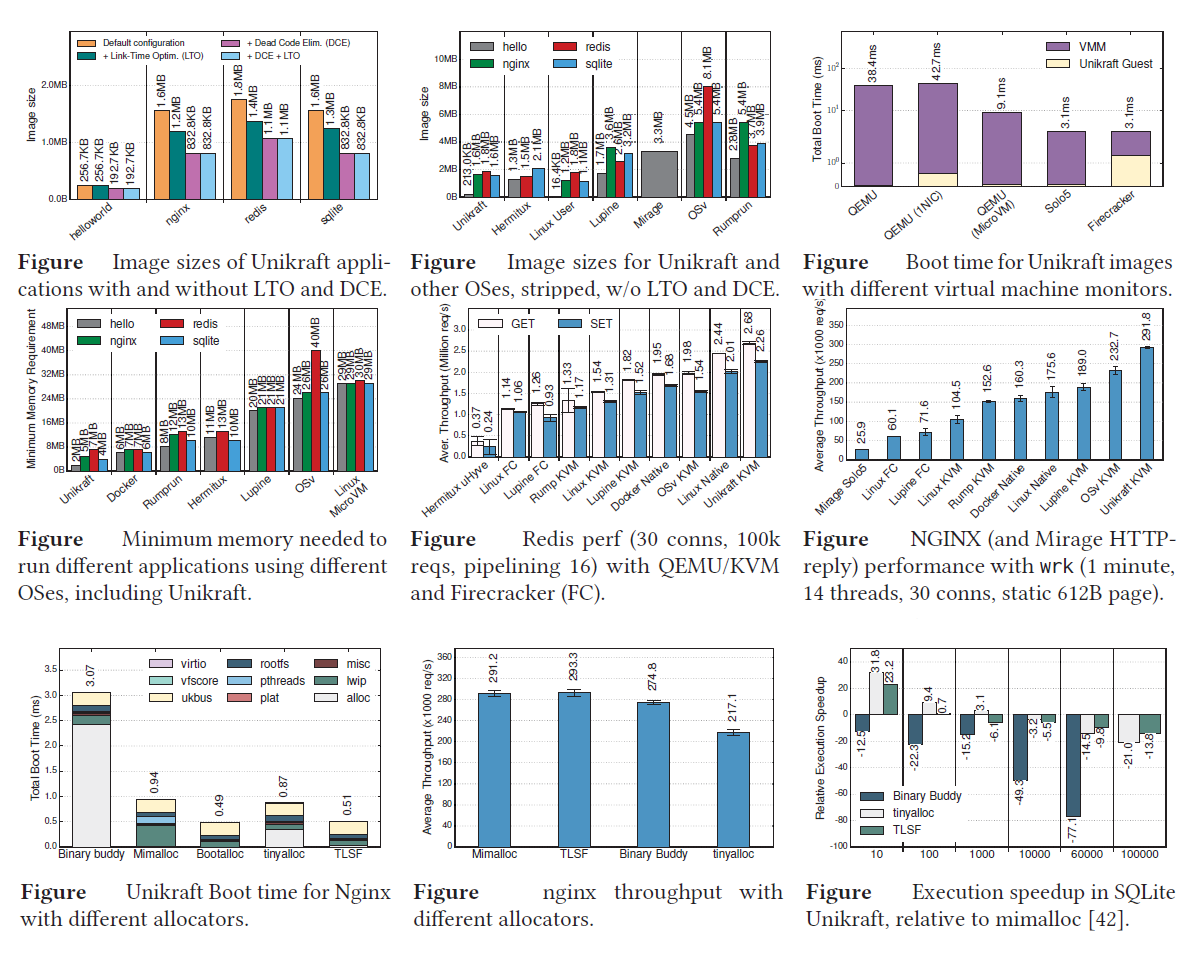
\includegraphics[width=.85\textwidth]{Figures/12.png}
\caption{Performance overview of Unikraft and comparison against competitors\cite{DEL14}}
\label{fig:6}
\end{figure}



The following experiments are done with a machine using Intel core I5 4500H 4 core CPU  clocked at 2.50 GHz, 8 gigabytes of ram. Primary operating systems were Ubuntu and CentOs depending on the situation. The system was freshly installed with Linux operating systems before each attempt. We tried to compile and test various open-source LWKs and Unikernels such as Azalea, HermitCore, mckernel, MirageOs, Unikraft.
Table \ref{table:2}  describes the summery of each experiment.



\begin{table}[htbp]
\resizebox{\columnwidth}{!}{
\begin{tabular}{ccccc}
\hline
 Kernel&Main Linux OS&Architecture&Status&Result \\ 
\hline
 Azalea & CentOs & x86 & Failed to install & Fail\\
 
 Hermitcore & Ubuntu & x86 & Failed to compile on machine  & Fail \\ 
 mckernel & CentOs & x86 & Failed to compile on machine & Fail \\ 
 mckernel & CentOs & arm64 & Failed to compile on machine & Fail \\ 
 MirageOs & Ubuntu & x86 & Successfully compiled on machine  & Partial Success \\ 
  &  & & but failed to boot anything other  &  \\ 
  &  & &  than helloworld &  \\ 
 MirageOs & RaspbianOS & arm64 & Failed to compile on machine & Fail \\ 
 Unikraft & Ubuntu & x86 & Successfully compiled and ran flask & Success\\
  &  & & server  &  \\ 
 Unikraft & RaspbianOS & arm64 & Successfully compiled on machine  & Partial Success \\ 
  &  & & but failed to boot anything other  &  \\ 
  &  & &  than helloworld &  \\ 
 
 
\hline
\end{tabular}}
\caption{Experiment with various kernels}
\label{table:2}
\end{table}


From Table \ref{table:2}, we can see that only Unikraft fully worked on our system. The rest of the kernels refused to compile or run. 

The biggest challenge we faced while trying to compile these kernels was a lack of support. Most of the guides the very difficult to follow. Moreover, if any error occurred, it was extremely difficult to debug because of the complex code struct and lack of supporting documents.  Furthermore, as our system was not officially supported, our failure rate was even high. We followed \cite{DEL22}, \cite{DEL23},\cite{DEL24}, \cite{DEL25}and \cite{DEL26}  to install  Azalea, HermitCore, mckernel, MirageOs, Unikraft respectively. Azalea, HermitCore, and mckernel failed to compile on our system. MirageOs and Unikraft compiled successfully but we could only run helloworld example on MirageOs. 

We followed "Python Flask on Unikraft" to install the Unikraft Flask server \cite{DEL18}. As unikraft specifically supports python 3.7.4, we had to manually install that version using pyenv \cite{DEL27}. We could then boot the Unikraft kernel using qemu kvm. We could not find any way to boot Unikraft natively on our system.


We also tried to compile and test the kernels mentioned above on the Raspberry pi 4 4 gigabyte model. Only helloworld module of Unikraft ran properly.  


We suspect such a situation occurred because these kernels are built for server CPUs such as Intel Xeon and Fujitsu A64FX \cite{DEL01} \cite{DEL02} \cite{DEL04}. Almost all of the LWKs and unikernels and specialized for servers, so it is understandable that consumer-grade CPUs are incompatible with them. So in the end, we were not able to fully implement the multikernel system. While we were able to boot unikraft it was not a true multikernel system as unikraft was running on kvm.


As only Unikrft ran properly on our main system, we will mainly focus on Unikraft. We have been able to run the flask server on Unikraft. While testing, the boot time of unikraft was found 3 seconds on average. Unikraft flask server consumes 60 milliwatts on average. On the other hand native Linux flask server process consumes 20 milliwatts on average. But if we also include Linux power consumption, the total power consumption will be 8000 milliwatts on average on a freshly booted system. For measuring power consumption, powerstat  \cite{DEL21} and PowerTOP \cite{DEL20} was used.

Figure~\ref{fig4} is the boot screen of Unikraft running Flask server.

Figure~\ref{fig5} is a comparison of power consumption between Unikraft Flask server and Linux native Flask server without including whole Linux power consumption. 


Figure~\ref{fig6} is a comparison of power consumption between Unikraft and Linux.


Unfortunately, due to a lack of proper hardware, we were unable to verify the full potential of the multikernel system. But this system still shows potential. Our experiment shows that this system uses less power if implemented properly. We have also seen from earlier work in \cite{DEL14} that this system also performs better in most cases. 



% ############################################################################
\section{Conclusions} \label{concl}
% ############################################################################


\subsection{Conclusions} 
In conclusion, multikernel system is a promising concept but needs more support. Previous work in \cite{DEL01} shows that 9\% to 280\% performance improvement was achieved using multikernel. In our experiment, we can see that Unikernel used 1/133 of power than Linux even while running on kvm. Though it was not running a true multikernel system, we can theoretically reduce power consumption drastically if we can implement a multikernel system properly. As this concept is relatively new, a lot of work needs to be done before this concept can mature. For now, most of the multikernel projects are open-source test projects. These are far from being stable. Currently, some kernels such as Unikraft, Include os, mirage os are receiving decent support but there is still room for improvement. As the support for these kernels gets better, they should also be more available to a wider range of systems. 
\subsection{Summary of Contributions}
In this paper, we tried to explore if the multikernel system is a viable alternative method to improve performance and battery life. We tried to test several mainstream sub kernels on consumer-level hardware such as generic laptops and raspberry pi. We also measured boot time and power consumption on Unikraft. But we could not boot anything meaningful on raspberry pi. As our main target system for the project is battery-powered devices, arm-powered raspberry pi should have been the main target system. Unfortunately, due to lack of support, raspberry pi was not able to boot anything that can be measured properly.
\subsection{Future Work}
Future work includes making multikernel systems more available and making them stable. To do that we need to make existing kernels work with more devices or create a new configurable kernel from the ground up with a large array of hardware support in mind. Previous work in \cite{DEL02} talks about hardware neutral multikernel, but we have not found anything that could be considered hardware neutral. Most kernels are intended for HPCs. The majority of the battery-powered devices have low-powered arm CPUs in them. So for this project goal to succeed, proper arm CPU support is necessary. As mentioned earlier, we also faced difficulty compiling some kernels on our system. In addition, proper support documents would be beneficial for trying, testing, and contributing to these projects. We faced a lot of issues while trying various kernels and the lack of a proper guide made it more challenging. Decent community and industry support would mitigate these issues. 



% ############################################################################
% Bibliography
% ############################################################################
\bibliographystyle{plain}
\bibliography{my-bibliography}     %loads my-bibliography.bib

% ============================================================================
\end{document}
% ============================================================================
